\section{Explicabilité additive multi-modèle inspirée de SHAP}
\label{sec:shap_framework}

Le premier cœur méthodologique des contributions du projet consiste à développer un \textit{framework} d'explicabilité capable d'analyser et de décomposer les forces structurantes qui régissent la formation des liens au sein d'un graphe. En s'inspirant de l'approche empirique de Ghasemian et al. \cite{01stackingLinkPred}, il reprend leur idée de combiner de nombreuses métriques et heuristiques d'horizon différents, en utilisant cette fois la prédiction de liens non pas comme une finalité, mais comme un instrument métrologique. Un méta-classificateur non linéaire de type (\textit{XGBoost}) est ensuite entraîné sur un vecteur de caractéristiques hétérogènes (topologiques, communautaires et géométriques) calculées sur le graphe. Enfin,  la théorie des jeux coopératifs permet d'isoler l'impact marginal de chaque paradigme.

\subsection{Protocole d'apprentissage rigoureux et étanchéité des données}

La prédiction de liens est par nature sujette au risque de fuite d'information (\textit{data leakage}), notamment lors du calcul de métriques de chemins ou d'espaces latents qui dépendent de la topologie globale. Pour garantir la validité statistique des résultats, un protocole d'échantillonnage strict est mis en place :

\begin{enumerate}
    \item \textbf{Ensemble d'Évaluation Externe ($10\,\%$):} Dès l'initialisation, $10\,\%$ des arêtes réelles du graphe original $G$ sont retirées et mises de côté (dans le graphe $G_{\text{hidden}}$) pour obtenir le graphe $G_{\text{kept}}$. Elles sont complétées par un échantillonnage de non-liens selon un ratio de $1$ pour $51$ pour constituer le \text{hidden\_set}, cohérent avec la sparsité (\textit{sparsity}) de la majorité des graphes réels. Les différentes métriques et heuristiques de ce dataset sont calculées à partir de la topologie de $G_{\text{kept}}$. Cet ensemble est strictement mis de côté et ne sert qu'à la mesure finale des performances.
    \item \textbf{Ensemble d'entrainement $15\,\%$):} Sur le graphe résiduel $G_{\text{kept}}$, un second tirage aléatoire extrait $15\,\%$ de liens (mis de côté dans le graphe $G_{\text{test}}$) pour constituer le graphe $G_{\text{train}}$ avec donc $75\,\%$ des liens initiaux. Les liens de $G_{\text{test}}$ sont complétés par des non-liens selon un ratio de $1$ pour $11$ pour créer le \text{train\_set}, sur lequel les métriques sont calculées à partir de la topologie de $G_{\text{train}}$. C'est sur cet ensemble que le modèle \textit{XGBoost} sera entraîné.
    \item \textbf{k-fold cross-validation:} A partir du graphe résiduel $G_{\text{kept}}$ contenant $90\,\%$ des liens initiaux, une k-fold cross validation est effectuée, en prenant à chauqe fois $15\,\%$ comme ratio pour le test set. Cette phase permet l'optimisation des hyperparamètres de l'algorithme \textit{XGBoost}, avec $k$ fixé à $2$ dans nos simulations mais généralisable à $5$.
\end{enumerate}

\subsection{Agrégation additive des contributions par valeurs de Shapley}

Une fois le modèle \textit{XGBoost} final ajusté, l'approche SHAP (\textit{SHapley Additive exPlanations}) permet de calculer les contributions locales de chaque métrique pour chaque paire de nœuds $(u, v)$. En pratique, la complexité de calcul de ces SHAP-valeurs est exponentielle, les résultats présentés dans ce rapport utilisent donc le code optimisé pour les arbres proposés par la librairie SHAP.

Soient $\mathcal{C}_{\text{Topo}}$, $\mathcal{C}_{\text{Commu}}$ et $\mathcal{C}_{\text{Embed}}$ les ensembles d'attributs correspondant respectivement aux métriques topologiques brutes, aux modèles de blocs/communautés et aux coordonnées géométriques latentes. En vertu de l'axiome d'additivité de Shapley, la contribution locale d'un paradigme $K$ pour le lien $(u,v)$ s'obtient par sommation directe :
\begin{equation}
    \Phi_K(x_{uv}) = \sum_{i \in \mathcal{C}_K} \phi_i(x_{uv}) \quad \text{où} \quad K \in \{\text{Topo}, \text{Commu}, \text{Embed}\}
\end{equation}

L'explicabilité \textit{globale} à l'échelle du réseau complet est ensuite calculée en moyennant les valeurs absolues des contributions locales sur un ensemble des paires de noeuds d'évaluation, révélant ainsi la force structurante dominante du graphe.

\subsection{Validation du modèle à partir des vérités de terrain (\textit{Ground Truth})}
\label{sec:validation_gt}

Avant de confronter le \textit{framework} d'explicabilité aux métriques et algorithmes inférés de la littérature, il est indispensable de valider son fonctionnement sur les variables génératrices brutes ayant servi à construire le \textit{benchmark}. Cette étape intermédiaire permet de vérifier que le méta-classificateur \textit{XGBoost} puis le calcul de valeurs de Shapley sont mathématiquement capables de refléter le ratio d'hybridation $\alpha$ lorsqu'il est alimenté par une source d'information parfaite.

Pour ce faire, l'espace des caractéristiques est restreint pour chaque paire de noeuds à deux variables, directement issues des modèles de génération des graphes (non-DC) :
\begin{itemize}
    \item \textbf{GT\_pos :} La distance euclidienne exacte $d_{uv}$ entre chaque paire de nœuds au sein de l'espace latent original du modèle spatial.
    \item \textbf{GT\_sbm :} La probabilité théorique d'inter-connectivité de bloc, déterminée par la densité de la matrice SBM d'origine associée au couple de communautés auquelles appartiennent les nœuds $u$ et $v$.
\end{itemize}

L'analyse quantitative, détaillée au sur la Figure ~\ref{fig1}, synthétise l'évolution des contributions SHAP globales moyennes ($\Phi_{\text{GT\_pos}}$ et $\Phi_{\text{GT\_sbm}}$) obtenues sur les $11$ réseaux du \textit{benchmark} en faisant varier le ratio nominal $\alpha$ de $0.0$ (graphe spatial pur) à $1.0$ (graphe communautaire pur) par pas de $0.1$. Les valeurs de Shapley pouvant être positives (quand un facteur encourage la formation de lien) comme négatives (quand il le décourage), c'est sur leur valeur absolue moyenne à l'échelle du graphe qui y est mesurée.

Les résultats numériques confirment une dynamique parfaitement corrélée aux paramètres générateurs. Sur le graphe purement géométrique ($\alpha = 0.0$), l'explication est massivement dominée par la distance spatiale brute avec une contribution $\Phi_{\text{GT\_pos}} = 2,1644$, tandis que la structure de bloc est quasi-inexistante ($\Phi_{\text{GT\_sbm}} = 0,2317$). À mesure que le signal communautaire est injecté, on observe une décroissance presque linéaire et monotone de la contribution spatiale, qui atteint son minimum de $0,3167$ à $\alpha = 1.0$. Symétriquement, la variable $\text{GT\_sbm}$ suit une trajectoire miroir croissante, atteignant un maximum sur le graphe communautaire pur avec un score de $2,2268$. Lorsque l'hybridation est équilibrée ($\alpha = 0.5$), les SHAP valeurs des 2 \textit{Ground Truths} sont équivalentes.

Ces résultats valident empiriquement la capacité du couplage entre le prédicteur \textit{XGBoost} et le calcul de valeurs de Shapley à décoder et retranscrire la nature des forces structurantes du graphe. Le framework se comportant comme un instrument de mesure neutre et robuste face à des variables théoriques parfaites, nous pouvons désormais déployer cette méthodologie sur les métriques et algorithmes de l'état de l'art afin d'en analyser les mécanismes d'inférence.


\begin{figure}
\includegraphics[width=\textwidth]{Plots/20 SHAPvals_GT_evolution_sbmv4.png}
\caption{Évolution des contributions SHAP globales moyennes de la \textit{Ground Truth} en fonction du ratio d'hybridation $\alpha$ (sur 10 expérimentations)} \label{fig1}
\end{figure}

\subsection{Application du modèle aux métriques et algorithmes de l'état de l'Art}

La même méthodologie est cette fois appliquée sur 22 métriques et algorithmes classiquement utilisés dans l'état de l'art, détaillés plus en détail en Annexe 2 (\ref{sec:Annexe2}). Elles sont regroupées en 3 grands paradigmes:
\begin{itemize}
    \item \textbf{Topologiques :} degree, pr, ppr, lcc, and, dc, katz, cn, aa, ra, jc, pa, sp
    \item \textbf{Communautés :} louvain, infomap, sbm, leiden, surprise, significance
    \item \textbf{Plongements géométriques (\textit{Embeddings}):} deepwalk, n2v\_homophily, crosswalk
\end{itemize}

\subsubsection{Analyse par paradigme}
\begin{figure}
\includegraphics[width=\textwidth]{Plots/203 SHAPvals_AllMetrics_evolution_sbmv4.png}
\caption{Evolution de l'importance des features regroupées par paradigme par additivité (moyenne sur 10 itérations), avec intervalle de confiance à 95\%.} \label{fig2}
\end{figure}

Une première analyse globale proposée consiste à calculer la moyenne de la valeur absolue des SHAP valeurs de chaque features (sur 10 itérations), puis à les regrouper par paradigme par additivité. Les courbes obtenues, synthétisées en Figure \ref{fig2}, révèlent qu'aucun paradigme ne domine pour toutes les valeurs de $\alpha$. La stochasticité y est forte, en raison du mécanisme de \textit{sampling} du calcul des SHAP valeurs dont la complexité est sinon exponentielle. L'analyse des courbes permet tout de même de dégager plusieurs tendances : 

L'importance globale du paradigme des \textbf{plongements géométriques} (\textit{Embeddings}) montre une grande stabilité  sur l'ensemble des ratios d'hybridation, oscillant de manière quasi-constante autour d'une valeur de $1,0$. Cette absence de sensibilité aux variations de $\alpha$ suggère une forte polyvalence de ces représentations latentes. Les algorithmes basés sur des marches aléatoires (\textit{Skip-gram}) semblent parvenir à capturer de l'information utile quelle que soit sa nature, géométrique ou communautaire. Cette capacité pourrait toutefois induire de la redondance entre ces métriques et d'autres.

À l'inverse, les caractéristiques issues des \textbf{algorithmes de communautés} et du \textbf{paradigme topologique} décrivent des trajectoires concaves, étant plus utilisées par le modèle aux extrémités du \textit{benchmark} ($\alpha \rightarrow 0$ et $\alpha \rightarrow 1$). Un paradoxe marquant émerge cependant aux bornes : sur un graphe purement spatial ($\alpha = 0,0$), l'approche communautaire obtient l'attribution la plus élevée ($1,4245 \pm 0,3273$), surpassant sa propre contribution sur un graphe purement communautaire ($1,0609 \pm 0,1962$ à $\alpha = 1,0$). Ce comportement contre-intuitif confirme l'existence d'un biais d'interprétation : les algorithmes de détection de blocs semblent capturer les densités locales créées par la proximité géographique, qu'ils traduisent à tort comme une structure de communauté. Ce fonctionnement ne pose pas de problème pour la prédiction de lien pure, mais nuance leur interprétabilité.

\subsubsection{Analyse des features individuelles}

Une analyse plus ciblée des contributions individuelles confirme et précise les dynamiques observées à l'échelle des paradigmes. La carte thermique des valeurs SHAP du top 10 des caractéristiques les plus influentes (Figure~\ref{fig3}) permet de visualiser la répartition détaillée de l'attribution. Une vue exhaustive intégrant l'ensemble des variables significativement exploitées (top 20) est reportée en Annexe~\ref{sec:Annexe3}.

\begin{figure}
\includegraphics[width=\textwidth]{Plots/201 SHAPvals_top10_heatmap_sbmv4.png}
\caption{Evolution de l'importance du top 10 métriques, mesurée à travers la valeur absolue moyenne de leurs SHAP valeurs sur le dataset d'évluation (sur 10 itérations).} \label{fig3}
\end{figure}

Ces résultats confirment que les méthodes d'inférences de communautés (ex : Surprise, Significance) sont plus utilisées par le modèle \textit{XGBoost} pour des valeurs marquées de $\alpha$ proche de $0$ ou $1$, mettant en exergue le besoin connu des méthodes d'inférence de communautés de la présence d'un signal fort pour fonctionner efficacement. Les métriques associées aux plongements vectoriels (n2v\_homophily\_cos, crosswalk\_cos) ont des SHAP valeurs plus stables, et de façon intéressantes c'est la cosine similarity qui a été préférée à la distance euclidienne brute.

Ils révèlent également un phénomène d'extinction, produit de l'effet combiné de l'apprentissage par arbres de décision de \textit{XGBoost} et de la méthode d'approximation de \textit{TreeSHAP} en présence de colinéarité. Lorsque plusieurs variables apportent une information redondante, le classificateur privilégie de manière opportuniste l'une d'entre elles lors des coupures (\textit{splits}). L'algorithme \textit{TreeSHAP}, calculant les contributions marginales à travers les chemins de décision construits par le modèle, hérite de ce masquage et attribue l'essentiel de l'importance à la variable sélectionnée, réduisant ainsi artificiellement la contribution SHAP des autres descripteurs colinéaires

Il est très visible au sein de la catégorie communautaire, dont l'évaluation montre que les métriques de densité basées sur \textit{Surprise} (\texttt{surprise\_density}) et \textit{Significance} (\texttt{significance\_density}) capturent l'essentiel de l'attribution sur la zone spatiale ($\alpha \le 0,3$). La matrice de connectivité du modèle en blocs stochastiques (\texttt{sbm\_density}) prend ensuite le relais sur la zone à fort signal de blocs ($\alpha \ge 0,5$), atteignant son apogée à $\alpha = 0,9$ ($0,4076$). Des algorithmes majeurs comme \texttt{louvain} ou \texttt{leiden} se retrouvent ainsi statistiquement invisibles dans ce top 10 : leurs partitions étant alignées avec celles de \textit{Surprise} ou de \textit{SBM}, le modèle concentre ses gains SHAP sur un nombre restreint de descripteurs cibles.

\subsection{Polyvalence géométrico-structurelle des métriques}

\begin{figure}
\includegraphics[width=\textwidth]{Plots/204bis 00_perfs_AllMetrics_artificial_graph_sbmv_4_10iter_20260527s_AUC-ROC_eval_CI99_SBM_ratio.png}
\caption{Evolution de l'AUC-ROC du modèle de prédiction de lien \protect\textit{XGBoost} entraîné à l'aide des feature Topologiques, Communautaires ou \protect\textit{Embeddings}, avec pour référence la meilleure performance théoriquement atteignable (sur 10 itérations).}
\label{fig 7}
\end{figure}

Idéalement, les variables d'embeddings ne devraient s'activer que sur les configurations spatiales ($\alpha \rightarrow 0$), et les variables communautaires sur les configurations en blocs ($\alpha \rightarrow 1$). Or, l'expérimentation montre que les plongements géométriques (\textit{embeddings}) s'avèrent extrêmement performants pour capturer les structures de blocs, tandis que les algorithmes de communautés s'ajustent efficacement sur les densités locales des modèles spatiaux. L'analyse des courbes de performance de prédiction de liens par groupe (Figure \ref{fig 7}) confirme cette limite théorique majeure, agissant comme le pivot scientifique de ce stage. 

Cette observation empirique est confirmée par notre étude statistique de corrélation entre les features géométriques et communautaires, et les vérités terrain (Figure \ref{fig5}). Les features géométriques et communautaires sont plus corrélées à la \textit{GroundTruth} spatiale quand c'est l'origine prédominante du graphe hybride ($\alpha < 0.5$), et à la \textit{GroundTruth} communautaire dans le cas contraire ($\alpha > 0.5$). Cette corrélation est également vérifiée par une analyse non linéaire basée sur l'Information Mutuelle (Annexe \ref{sec:Annexe4}).

\begin{figure}
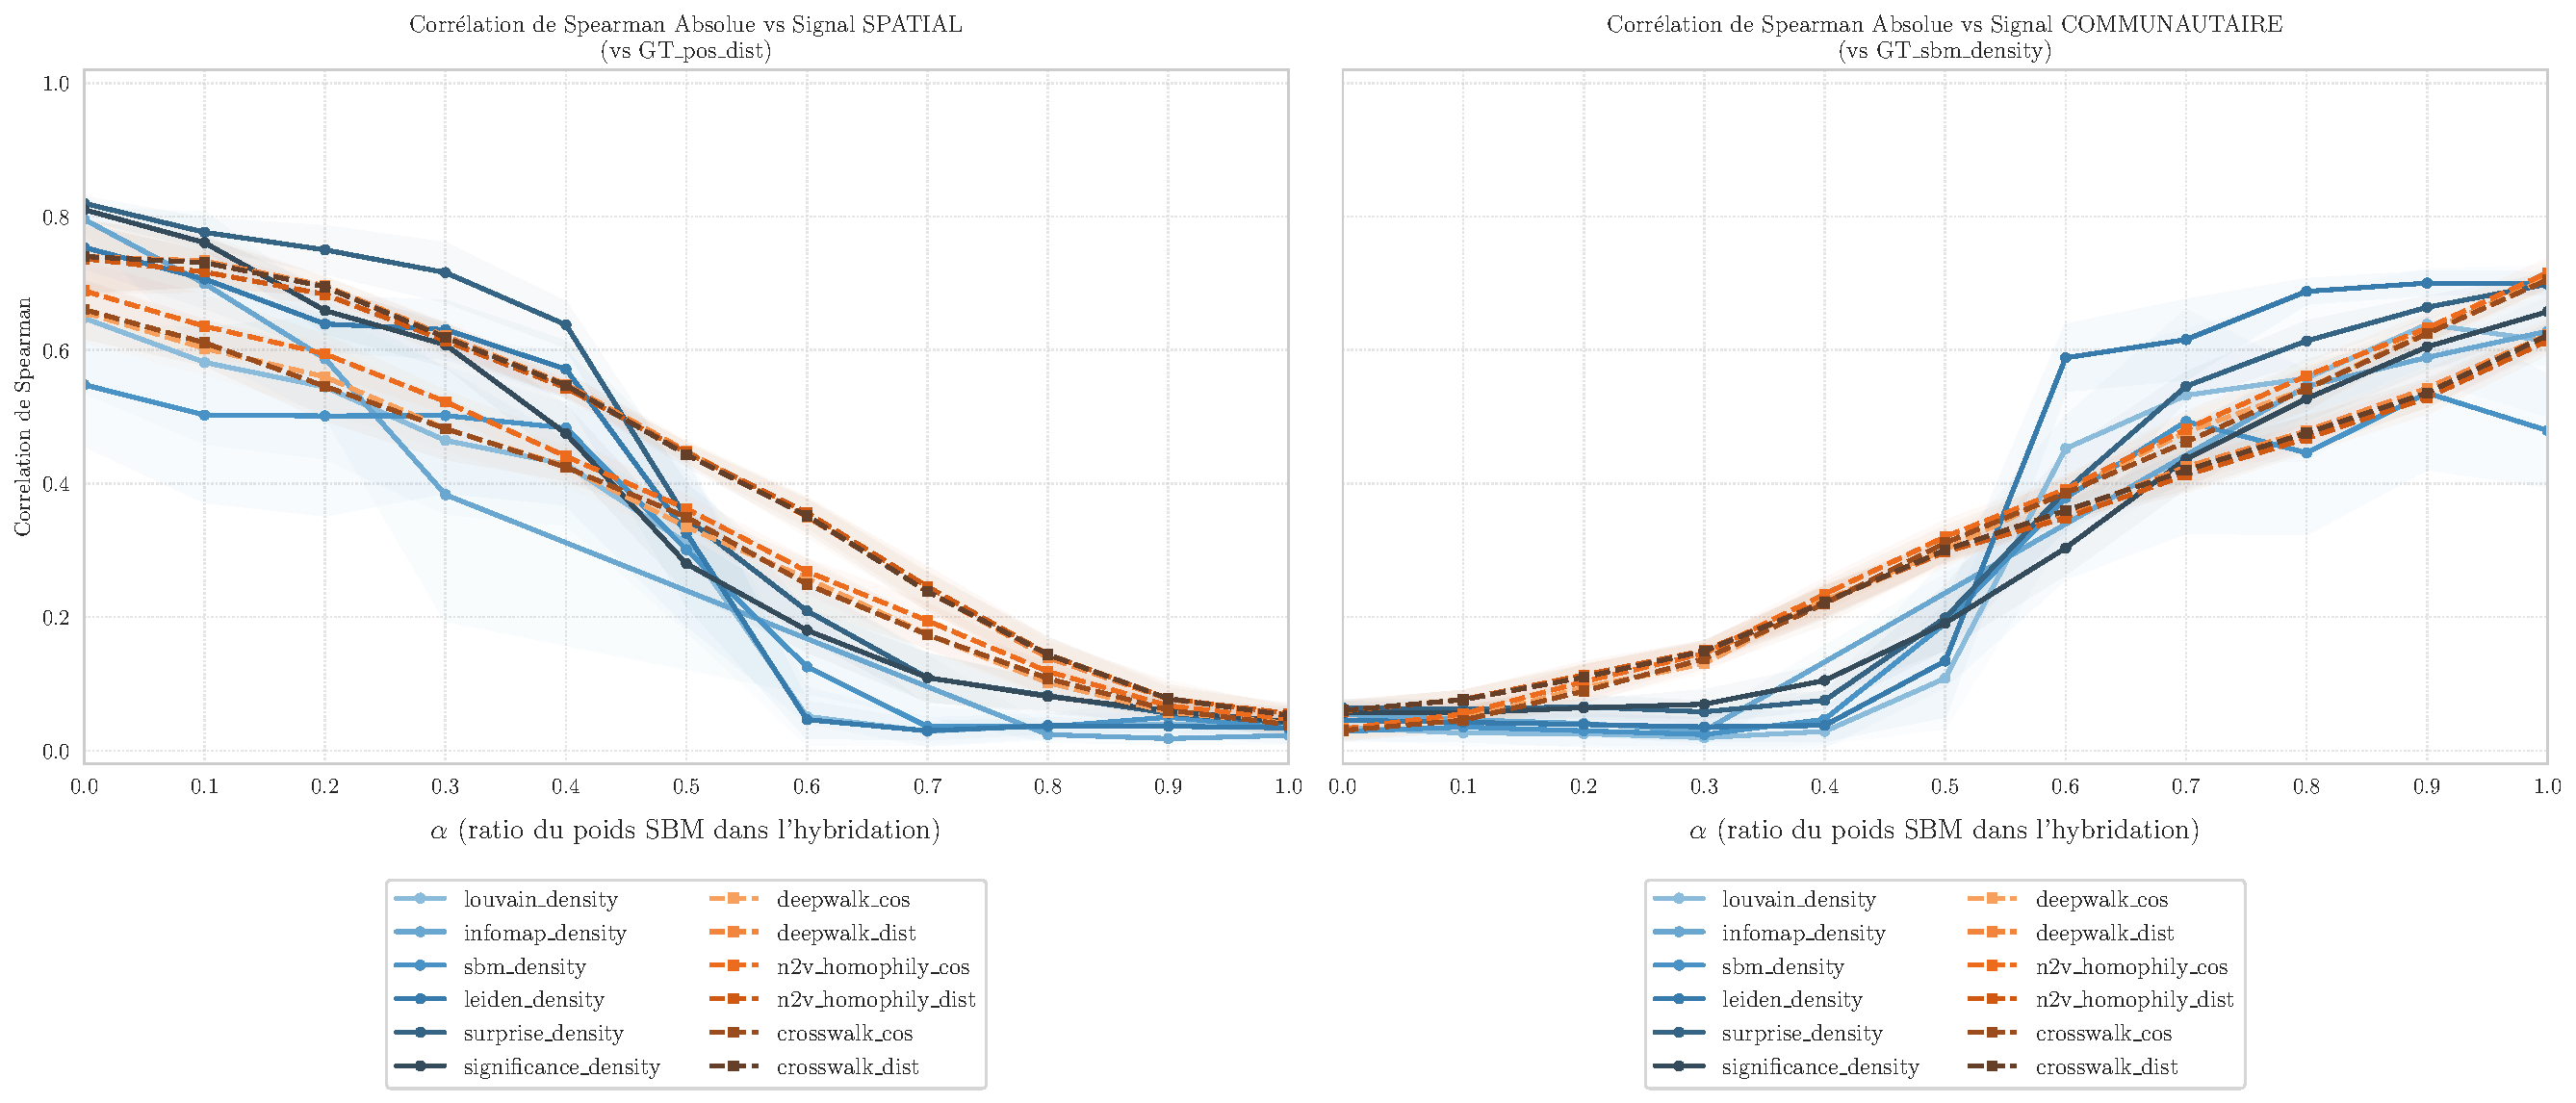
\includegraphics[width=\textwidth]{Plots/206 00_Correl_individual_features_VS_GT_comparison.pdf}
\caption{Evolution du coefficient de spearman entre les features et la \textit{Ground Truth} communautaire (à droite), et la \textit{Ground Truth} géométrique (à gauche) en fonction de $\alpha$ (moyenne sur 10 itérations).} 
\label{fig5}
\end{figure}


\subsection{Redondance entre les descripteurs Communautaires et \textit{Embeddings}}

Cette polyvalence géométrico-structurelle traduit également le fait que ces deux familles de descripteurs souffrent d'une forte redondance informationnelle. Afin de quantifier précisément ce chevauchement, le Tableau~\ref{tab:collinearity_alpha} synthétise l'évolution de la corrélation de Spearman moyenne calculée sur l'ensemble des paires de caractéristiques issues des paradigmes communautaire et géométrique ($6 \times 6$ paires car 6 variables pour chaque paradigme).

\begin{table}[!ht]
\centering
\caption{Évolution de la colinéarité moyenne inter-paradigme (Spearman) en fonction de $\alpha$ avec un intervalle de confiance à 95\,\% (10 itérations)}
\label{tab:collinearity_alpha}
\begin{tabular}{cc}
\hline
\textbf{Ratio SBM ($\alpha$)} & \textbf{Corrélation Moyenne Inter-Groupe $|\rho| \pm \text{IC}_{95\%}$} \\
\hline
1,0 & 0,6166 $\pm$ 0,0210 \\
0,9 & 0,5392 $\pm$ 0,0205 \\
0,8 & 0,4409 $\pm$ 0,0143 \\
0,7 & 0,3993 $\pm$ 0,0068 \\
0,6 & 0,3403 $\pm$ 0,0111 \\
0,5 & 0,3133 $\pm$ 0,0072 \\
0,4 & 0,3978 $\pm$ 0,0125 \\
0,3 & 0,4535 $\pm$ 0,0250 \\
0,2 & 0,5157 $\pm$ 0,0182 \\
0,1 & 0,5768 $\pm$ 0,0134 \\
0,0 & 0,6330 $\pm$ 0,0184 \\
\hline
\end{tabular}
\end{table}

Son analyse montre que la colinéarité inter-groupe décrit une courbe convexe symétrique, atteignant un minimum à $\alpha = 0,5$ avec une corrélation absolue moyenne de $0,3133 \pm 0,0072$. À mesure que le réseau se polarise vers l'un des deux générateurs purs, cette corrélation s'exacerbe et devient hautement significative, culminant à $0,6166 \pm 0,0210$ pour le pôle communautaire ($\alpha = 1,0$) et jusqu'à $0,6330 \pm 0,0184$ pour le pôle spatial ($\alpha = 0,0$). 

Cette colinéarité floute l'explicabilité du modèle en introduisant un effet de confusion : le méta-classificateur ne sépare pas des signaux orthogonaux indicateurs d'un facteur spécifique. Ce verrou méthodologique justifie directement l'introduction, dans le chapitre suivant, de nos approches d'inférence de métriques décorrélées par débiaisage géométrique.

